\documentclass[11pt,a4paper]{article}

\newcommand{\doctitle}{Depth-Damage Curve Model (MKM-DD-001)}
\newcommand{\docsubtitle}{Wolfram Oracle Benchmark of the Flood Risk Model Document}
\newcommand{\docversion}{0.1}
\newcommand{\docdate}{03-November-2026}
\newcommand{\docauthor}{David K Kelly}

% MKM Research Labs — Shared Document Header
% Usage: % MKM Research Labs — Shared Document Header
% Usage: % MKM Research Labs — Shared Document Header
% Usage: \input{../shared/mkm_header}  (before \begin{document})
%
% Required commands before \input:
%   \newcommand{\doctitle}{...}
%   \newcommand{\docsubtitle}{...}
%   \newcommand{\docversion}{1.0}
%   \newcommand{\docdate}{13-February-2026}
%   \newcommand{\docauthor}{David K Kelly}

% ─── Packages ───────────────────────────────────────────────────────────────
\usepackage[utf8]{inputenc}
\usepackage{amsmath,amsfonts,amssymb}
\usepackage{listings}
\usepackage{color,xcolor}
\usepackage{graphicx}
\usepackage{hyperref}
\usepackage[toc,page]{appendix}
\usepackage{tabto}
\usepackage{float}
\usepackage{comment}
\usepackage[en-GB]{datetime2}
\usepackage{setspace}
\usepackage{subcaption}
\usepackage{booktabs}
\usepackage{longtable}
\usepackage{adjustbox}
\usepackage{enumitem}
\usepackage{fancyhdr}
\usepackage{lastpage}

% ─── Page geometry ──────────────────────────────────────────────────────────
\onehalfspacing
\usepackage{geometry}
\geometry{a4paper, total={170mm,247mm}, left=20mm, top=25mm, bottom=25mm}

% ─── Headers and footers ───────────────────────────────────────────────────
\pagestyle{fancy}
\fancyhf{}
\fancyhead[L]{\small\textcolor{gray}{MKM Research Labs}}
\fancyhead[R]{\small\textcolor{gray}{\doctitle{} --- v\docversion}}
\fancyfoot[C]{\small\textcolor{gray}{CONFIDENTIAL}}
\fancyfoot[R]{\small\textcolor{gray}{Page \thepage\ of \pageref{LastPage}}}
\renewcommand{\headrulewidth}{0.4pt}
\renewcommand{\footrulewidth}{0.4pt}

% ─── Colours ────────────────────────────────────────────────────────────────
\definecolor{mkmblue}{HTML}{1565C0}
\definecolor{codegreen}{rgb}{0,0.6,0}
\definecolor{codegray}{rgb}{0.5,0.5,0.5}
\definecolor{codepurple}{rgb}{0.58,0,0.82}
\definecolor{backcolour}{rgb}{0.95,0.95,0.92}

% ─── Hyperref setup ─────────────────────────────────────────────────────────
\hypersetup{
    colorlinks=true,
    linkcolor=mkmblue,
    citecolor=mkmblue,
    urlcolor=mkmblue
}

% ─── Code listings ──────────────────────────────────────────────────────────
\lstdefinestyle{mystyle}{
    backgroundcolor=\color{backcolour},
    commentstyle=\color{codegreen},
    keywordstyle=\color{magenta},
    numberstyle=\tiny\color{codegray},
    stringstyle=\color{codepurple},
    basicstyle=\ttfamily\footnotesize,
    breakatwhitespace=false,
    breaklines=true,
    captionpos=b,
    keepspaces=true,
    numbers=left,
    numbersep=5pt,
    showspaces=false,
    showstringspaces=false,
    showtabs=false,
    tabsize=2
}
\lstset{style=mystyle}

% ─── Section formatting ────────────────────────────────────────────────────
\setcounter{tocdepth}{3}
\setcounter{secnumdepth}{3}

% ─── Shared macros ──────────────────────────────────────────────────────────
\newcommand{\mkmtitlepage}{%
    \begin{titlepage}
    \begin{center}
    \vspace*{1cm}
    \begin{figure}[H]\centering
        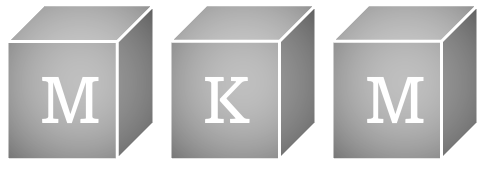
\includegraphics[width=0.4\textwidth]{../shared/Logos/MKM_logo.png}
    \end{figure}
    \vspace{1.5cm}
    {\Huge\bfseries\textcolor{mkmblue}{\doctitle}\par}
    \vspace{0.5cm}
    {\Large\textcolor{gray}{\docsubtitle}\par}
    \vspace{2cm}
    {\large MKM Research Labs\par}
    \vspace{0.5cm}
    {\large Version \docversion{} --- \docdate\par}
    \vspace{0.5cm}
    {\large \docauthor\par}
    \vspace{2cm}
    \textcolor{red}{\textbf{CONFIDENTIAL --- PROPRIETARY}}
    \end{center}
    \end{titlepage}
}

\newcommand{\mkmlegalpage}{%
    \clearpage
    \thispagestyle{empty}
    \begin{center}
    \large\textbf{Legal Notice}
    \vspace{1em}

    \textbf{PROPRIETARY AND CONFIDENTIAL}
    \end{center}

    \noindent This document, including all algorithms, models, methodology, formulas,
    calculations, and intellectual concepts contained herein, constitutes the exclusive
    intellectual property and confidential trade secrets of MKM Research Labs (``MKM'').

    \vspace{0.5em}
    \noindent Any usage, reproduction, distribution, modification, or disclosure of this
    document or any portion thereof, without the express prior written authorisation from
    MKM Research Labs is strictly prohibited and constitutes an infringement of intellectual
    property rights.

    \vspace{0.5em}
    \noindent The document is provided on an ``as is'' basis. MKM Research Labs makes no
    representations or warranties of any kind, express or implied, regarding its accuracy,
    reliability, or suitability for any particular purpose.

    \vspace{1em}
    \begin{center}
    All rights reserved. \copyright\ 2021--2026 MKM Research Labs.

    \vspace{0.5em}
    Governed by the laws of the United Kingdom.
    \end{center}
    \clearpage
}

\newcommand{\mkmhistorypage}[1]{%
    \section{Document History}
    \begin{table}[ht]
        \centering
        \begin{tabular}{l|l|l|l}
            \textbf{Date} & \textbf{Version} & \textbf{Description} & \textbf{Author} \\
            \hline
            #1
        \end{tabular}
        \label{tab:revision_history}
    \end{table}
    \clearpage
}

% ─── Bank validation protocol section commands ──────────────────────────────
% Use these to ensure every model doc has the required sections.
% They are just styled \section calls — content is provided by each doc.

\newcommand{\mkmexecsummary}{\section{Executive Summary}}
\newcommand{\mkmpurpose}{\section{Model Purpose and Scope}}
\newcommand{\mkmframework}{\section{Mathematical Framework}}
\newcommand{\mkminputs}{\section{Input Parameters and Calibration}}
\newcommand{\mkmimplementation}{\section{Implementation Details}}
\newcommand{\mkmsensitivity}{\section{Sensitivity Analysis}}
\newcommand{\mkmvalidation}{\section{Validation and Backtesting}}
\newcommand{\mkmtestresults}{\subsection{Automated Test Results}\input{test_results}}
\newcommand{\mkmlimitations}{\section{Model Limitations and Known Weaknesses}}

\newcommand{\mkmgovernance}{\section{Governance Validation Questions}
\noindent The following nine questions are mandated by Chapter~5 of the
\emph{Model Risk Governance for Vendors} handbook and must be explicitly
addressed for every model in the inventory. Response status is tracked in the
Model Governance Dashboard (MRC portal). \par\medskip}

\newcommand{\mkmvqitem}[3]{\subsection{Q#1 --- #2}
\noindent\textit{``#3''}\par\medskip\noindent}

\newcommand{\mkmchangelog}{\section{Change History}}
  (before \begin{document})
%
% Required commands before \input:
%   \newcommand{\doctitle}{...}
%   \newcommand{\docsubtitle}{...}
%   \newcommand{\docversion}{1.0}
%   \newcommand{\docdate}{13-February-2026}
%   \newcommand{\docauthor}{David K Kelly}

% ─── Packages ───────────────────────────────────────────────────────────────
\usepackage[utf8]{inputenc}
\usepackage{amsmath,amsfonts,amssymb}
\usepackage{listings}
\usepackage{color,xcolor}
\usepackage{graphicx}
\usepackage{hyperref}
\usepackage[toc,page]{appendix}
\usepackage{tabto}
\usepackage{float}
\usepackage{comment}
\usepackage[en-GB]{datetime2}
\usepackage{setspace}
\usepackage{subcaption}
\usepackage{booktabs}
\usepackage{longtable}
\usepackage{adjustbox}
\usepackage{enumitem}
\usepackage{fancyhdr}
\usepackage{lastpage}

% ─── Page geometry ──────────────────────────────────────────────────────────
\onehalfspacing
\usepackage{geometry}
\geometry{a4paper, total={170mm,247mm}, left=20mm, top=25mm, bottom=25mm}

% ─── Headers and footers ───────────────────────────────────────────────────
\pagestyle{fancy}
\fancyhf{}
\fancyhead[L]{\small\textcolor{gray}{MKM Research Labs}}
\fancyhead[R]{\small\textcolor{gray}{\doctitle{} --- v\docversion}}
\fancyfoot[C]{\small\textcolor{gray}{CONFIDENTIAL}}
\fancyfoot[R]{\small\textcolor{gray}{Page \thepage\ of \pageref{LastPage}}}
\renewcommand{\headrulewidth}{0.4pt}
\renewcommand{\footrulewidth}{0.4pt}

% ─── Colours ────────────────────────────────────────────────────────────────
\definecolor{mkmblue}{HTML}{1565C0}
\definecolor{codegreen}{rgb}{0,0.6,0}
\definecolor{codegray}{rgb}{0.5,0.5,0.5}
\definecolor{codepurple}{rgb}{0.58,0,0.82}
\definecolor{backcolour}{rgb}{0.95,0.95,0.92}

% ─── Hyperref setup ─────────────────────────────────────────────────────────
\hypersetup{
    colorlinks=true,
    linkcolor=mkmblue,
    citecolor=mkmblue,
    urlcolor=mkmblue
}

% ─── Code listings ──────────────────────────────────────────────────────────
\lstdefinestyle{mystyle}{
    backgroundcolor=\color{backcolour},
    commentstyle=\color{codegreen},
    keywordstyle=\color{magenta},
    numberstyle=\tiny\color{codegray},
    stringstyle=\color{codepurple},
    basicstyle=\ttfamily\footnotesize,
    breakatwhitespace=false,
    breaklines=true,
    captionpos=b,
    keepspaces=true,
    numbers=left,
    numbersep=5pt,
    showspaces=false,
    showstringspaces=false,
    showtabs=false,
    tabsize=2
}
\lstset{style=mystyle}

% ─── Section formatting ────────────────────────────────────────────────────
\setcounter{tocdepth}{3}
\setcounter{secnumdepth}{3}

% ─── Shared macros ──────────────────────────────────────────────────────────
\newcommand{\mkmtitlepage}{%
    \begin{titlepage}
    \begin{center}
    \vspace*{1cm}
    \begin{figure}[H]\centering
        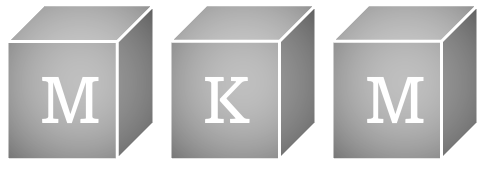
\includegraphics[width=0.4\textwidth]{../shared/Logos/MKM_logo.png}
    \end{figure}
    \vspace{1.5cm}
    {\Huge\bfseries\textcolor{mkmblue}{\doctitle}\par}
    \vspace{0.5cm}
    {\Large\textcolor{gray}{\docsubtitle}\par}
    \vspace{2cm}
    {\large MKM Research Labs\par}
    \vspace{0.5cm}
    {\large Version \docversion{} --- \docdate\par}
    \vspace{0.5cm}
    {\large \docauthor\par}
    \vspace{2cm}
    \textcolor{red}{\textbf{CONFIDENTIAL --- PROPRIETARY}}
    \end{center}
    \end{titlepage}
}

\newcommand{\mkmlegalpage}{%
    \clearpage
    \thispagestyle{empty}
    \begin{center}
    \large\textbf{Legal Notice}
    \vspace{1em}

    \textbf{PROPRIETARY AND CONFIDENTIAL}
    \end{center}

    \noindent This document, including all algorithms, models, methodology, formulas,
    calculations, and intellectual concepts contained herein, constitutes the exclusive
    intellectual property and confidential trade secrets of MKM Research Labs (``MKM'').

    \vspace{0.5em}
    \noindent Any usage, reproduction, distribution, modification, or disclosure of this
    document or any portion thereof, without the express prior written authorisation from
    MKM Research Labs is strictly prohibited and constitutes an infringement of intellectual
    property rights.

    \vspace{0.5em}
    \noindent The document is provided on an ``as is'' basis. MKM Research Labs makes no
    representations or warranties of any kind, express or implied, regarding its accuracy,
    reliability, or suitability for any particular purpose.

    \vspace{1em}
    \begin{center}
    All rights reserved. \copyright\ 2021--2026 MKM Research Labs.

    \vspace{0.5em}
    Governed by the laws of the United Kingdom.
    \end{center}
    \clearpage
}

\newcommand{\mkmhistorypage}[1]{%
    \section{Document History}
    \begin{table}[ht]
        \centering
        \begin{tabular}{l|l|l|l}
            \textbf{Date} & \textbf{Version} & \textbf{Description} & \textbf{Author} \\
            \hline
            #1
        \end{tabular}
        \label{tab:revision_history}
    \end{table}
    \clearpage
}

% ─── Bank validation protocol section commands ──────────────────────────────
% Use these to ensure every model doc has the required sections.
% They are just styled \section calls — content is provided by each doc.

\newcommand{\mkmexecsummary}{\section{Executive Summary}}
\newcommand{\mkmpurpose}{\section{Model Purpose and Scope}}
\newcommand{\mkmframework}{\section{Mathematical Framework}}
\newcommand{\mkminputs}{\section{Input Parameters and Calibration}}
\newcommand{\mkmimplementation}{\section{Implementation Details}}
\newcommand{\mkmsensitivity}{\section{Sensitivity Analysis}}
\newcommand{\mkmvalidation}{\section{Validation and Backtesting}}
\newcommand{\mkmtestresults}{\subsection{Automated Test Results}\input{test_results}}
\newcommand{\mkmlimitations}{\section{Model Limitations and Known Weaknesses}}

\newcommand{\mkmgovernance}{\section{Governance Validation Questions}
\noindent The following nine questions are mandated by Chapter~5 of the
\emph{Model Risk Governance for Vendors} handbook and must be explicitly
addressed for every model in the inventory. Response status is tracked in the
Model Governance Dashboard (MRC portal). \par\medskip}

\newcommand{\mkmvqitem}[3]{\subsection{Q#1 --- #2}
\noindent\textit{``#3''}\par\medskip\noindent}

\newcommand{\mkmchangelog}{\section{Change History}}
  (before \begin{document})
%
% Required commands before \input:
%   \newcommand{\doctitle}{...}
%   \newcommand{\docsubtitle}{...}
%   \newcommand{\docversion}{1.0}
%   \newcommand{\docdate}{13-February-2026}
%   \newcommand{\docauthor}{David K Kelly}

% ─── Packages ───────────────────────────────────────────────────────────────
\usepackage[utf8]{inputenc}
\usepackage{amsmath,amsfonts,amssymb}
\usepackage{listings}
\usepackage{color,xcolor}
\usepackage{graphicx}
\usepackage{hyperref}
\usepackage[toc,page]{appendix}
\usepackage{tabto}
\usepackage{float}
\usepackage{comment}
\usepackage[en-GB]{datetime2}
\usepackage{setspace}
\usepackage{subcaption}
\usepackage{booktabs}
\usepackage{longtable}
\usepackage{adjustbox}
\usepackage{enumitem}
\usepackage{fancyhdr}
\usepackage{lastpage}

% ─── Page geometry ──────────────────────────────────────────────────────────
\onehalfspacing
\usepackage{geometry}
\geometry{a4paper, total={170mm,247mm}, left=20mm, top=25mm, bottom=25mm}

% ─── Headers and footers ───────────────────────────────────────────────────
\pagestyle{fancy}
\fancyhf{}
\fancyhead[L]{\small\textcolor{gray}{MKM Research Labs}}
\fancyhead[R]{\small\textcolor{gray}{\doctitle{} --- v\docversion}}
\fancyfoot[C]{\small\textcolor{gray}{CONFIDENTIAL}}
\fancyfoot[R]{\small\textcolor{gray}{Page \thepage\ of \pageref{LastPage}}}
\renewcommand{\headrulewidth}{0.4pt}
\renewcommand{\footrulewidth}{0.4pt}

% ─── Colours ────────────────────────────────────────────────────────────────
\definecolor{mkmblue}{HTML}{1565C0}
\definecolor{codegreen}{rgb}{0,0.6,0}
\definecolor{codegray}{rgb}{0.5,0.5,0.5}
\definecolor{codepurple}{rgb}{0.58,0,0.82}
\definecolor{backcolour}{rgb}{0.95,0.95,0.92}

% ─── Hyperref setup ─────────────────────────────────────────────────────────
\hypersetup{
    colorlinks=true,
    linkcolor=mkmblue,
    citecolor=mkmblue,
    urlcolor=mkmblue
}

% ─── Code listings ──────────────────────────────────────────────────────────
\lstdefinestyle{mystyle}{
    backgroundcolor=\color{backcolour},
    commentstyle=\color{codegreen},
    keywordstyle=\color{magenta},
    numberstyle=\tiny\color{codegray},
    stringstyle=\color{codepurple},
    basicstyle=\ttfamily\footnotesize,
    breakatwhitespace=false,
    breaklines=true,
    captionpos=b,
    keepspaces=true,
    numbers=left,
    numbersep=5pt,
    showspaces=false,
    showstringspaces=false,
    showtabs=false,
    tabsize=2
}
\lstset{style=mystyle}

% ─── Section formatting ────────────────────────────────────────────────────
\setcounter{tocdepth}{3}
\setcounter{secnumdepth}{3}

% ─── Shared macros ──────────────────────────────────────────────────────────
\newcommand{\mkmtitlepage}{%
    \begin{titlepage}
    \begin{center}
    \vspace*{1cm}
    \begin{figure}[H]\centering
        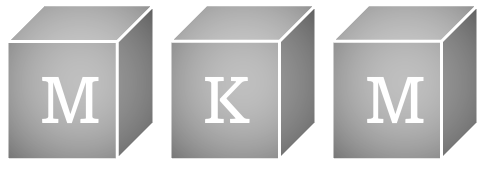
\includegraphics[width=0.4\textwidth]{../shared/Logos/MKM_logo.png}
    \end{figure}
    \vspace{1.5cm}
    {\Huge\bfseries\textcolor{mkmblue}{\doctitle}\par}
    \vspace{0.5cm}
    {\Large\textcolor{gray}{\docsubtitle}\par}
    \vspace{2cm}
    {\large MKM Research Labs\par}
    \vspace{0.5cm}
    {\large Version \docversion{} --- \docdate\par}
    \vspace{0.5cm}
    {\large \docauthor\par}
    \vspace{2cm}
    \textcolor{red}{\textbf{CONFIDENTIAL --- PROPRIETARY}}
    \end{center}
    \end{titlepage}
}

\newcommand{\mkmlegalpage}{%
    \clearpage
    \thispagestyle{empty}
    \begin{center}
    \large\textbf{Legal Notice}
    \vspace{1em}

    \textbf{PROPRIETARY AND CONFIDENTIAL}
    \end{center}

    \noindent This document, including all algorithms, models, methodology, formulas,
    calculations, and intellectual concepts contained herein, constitutes the exclusive
    intellectual property and confidential trade secrets of MKM Research Labs (``MKM'').

    \vspace{0.5em}
    \noindent Any usage, reproduction, distribution, modification, or disclosure of this
    document or any portion thereof, without the express prior written authorisation from
    MKM Research Labs is strictly prohibited and constitutes an infringement of intellectual
    property rights.

    \vspace{0.5em}
    \noindent The document is provided on an ``as is'' basis. MKM Research Labs makes no
    representations or warranties of any kind, express or implied, regarding its accuracy,
    reliability, or suitability for any particular purpose.

    \vspace{1em}
    \begin{center}
    All rights reserved. \copyright\ 2021--2026 MKM Research Labs.

    \vspace{0.5em}
    Governed by the laws of the United Kingdom.
    \end{center}
    \clearpage
}

\newcommand{\mkmhistorypage}[1]{%
    \section{Document History}
    \begin{table}[ht]
        \centering
        \begin{tabular}{l|l|l|l}
            \textbf{Date} & \textbf{Version} & \textbf{Description} & \textbf{Author} \\
            \hline
            #1
        \end{tabular}
        \label{tab:revision_history}
    \end{table}
    \clearpage
}

% ─── Bank validation protocol section commands ──────────────────────────────
% Use these to ensure every model doc has the required sections.
% They are just styled \section calls — content is provided by each doc.

\newcommand{\mkmexecsummary}{\section{Executive Summary}}
\newcommand{\mkmpurpose}{\section{Model Purpose and Scope}}
\newcommand{\mkmframework}{\section{Mathematical Framework}}
\newcommand{\mkminputs}{\section{Input Parameters and Calibration}}
\newcommand{\mkmimplementation}{\section{Implementation Details}}
\newcommand{\mkmsensitivity}{\section{Sensitivity Analysis}}
\newcommand{\mkmvalidation}{\section{Validation and Backtesting}}
\newcommand{\mkmtestresults}{\subsection{Automated Test Results}\input{test_results}}
\newcommand{\mkmlimitations}{\section{Model Limitations and Known Weaknesses}}

\newcommand{\mkmgovernance}{\section{Governance Validation Questions}
\noindent The following nine questions are mandated by Chapter~5 of the
\emph{Model Risk Governance for Vendors} handbook and must be explicitly
addressed for every model in the inventory. Response status is tracked in the
Model Governance Dashboard (MRC portal). \par\medskip}

\newcommand{\mkmvqitem}[3]{\subsection{Q#1 --- #2}
\noindent\textit{``#3''}\par\medskip\noindent}

\newcommand{\mkmchangelog}{\section{Change History}}

% T1 so the underscores in code identifiers print as underscores.
\usepackage[T1]{fontenc}
\usepackage{lmodern}
% Generated by tools.wolfram_oracle -- do not edit.
\newcommand{\bmGenerated}{2026-11-03}
\newcommand{\bmCodeCommit}{\texttt{7bbb63078a59}}
\newcommand{\bmCodeDirty}{}
\newcommand{\bmNumerics}{numpy 1.26.4, scipy 1.15.1, mpmath 1.4.1}
\newcommand{\bmWolfram}{15.0.0 for Mac OS X ARM (64-bit) (May 26, 2026)}
\newcommand{\bmWolframVia}{ via live kernel session (wolframclient)}
\newcommand{\bmWolframConfirms}{Wolfram, computing each independently, agrees with the reference to $4.1\times10^{-31}$.}
\newcommand{\bmChecks}{14}
\newcommand{\bmOutcome}{all pass}
\newcommand{\bmCodeErr}{$3.2\times10^{-16}$}
\newcommand{\bmZ}{1.82}
\newcommand{\bmVelocity}{2.19/1.37/0.91/0.55}
\newcommand{\bmShift}{1.064}
\newcommand{\bmDegErr}{61}
\newcommand{\bmEll}{10{,}000}
\newcommand{\bmDepthGap}{1.2}

% The shared history table sets every column to its natural width; wrap the description.
\renewcommand{\mkmhistorypage}[1]{%
    \section{Document History}
    \begin{table}[ht]
        \centering
        \begin{tabular}{l|l|p{9cm}|l}
            \textbf{Date} & \textbf{Version} & \textbf{Description} & \textbf{Author} \\
            \hline
            #1
        \end{tabular}
    \end{table}
}

\begin{document}
% Long code paths and identifiers cannot hyphenate; let the spacing stretch instead.
\sloppy

\mkmtitlepage
\mkmlegalpage

\tableofcontents
\clearpage

% =========================================================================
\mkmexecsummary
% =========================================================================

This document benchmarks the Depth-Damage Curve Model (MKM-DD-001), whose filed model
document is \emph{Flood Risk Model} (\texttt{flood\_risk.pdf}, v1.1, 18-Feb-2026). It
turns flood depth into a damage ratio, and carries the velocity, attenuation and
hydrograph functions that the property flood propagation and the hazard curve
builder use. It asks whether the code computes what the filed document says, and
whether what the document says holds.

\paragraph{The code computes the formulae it still implements.} The depth-damage curve,
Manning's velocity, slope, travel time, attenuation, haversine, IDW and correlation
matrix agree with a 50-digit implementation of the document's equations to
\bmCodeErr{}. The hydrograph agrees to the code's printed precision. The portfolio Monte
Carlo's mean loss is within \bmZ{} standard errors of the exact expected loss
(Table~\ref{tab:bm-checks}). Every printed figure in Tables~5--7 is reproduced.
\bmWolframConfirms

\paragraph{But the filed document no longer describes the model.} Its source has since
reached v1.4, which was never filed, and the code has moved past both
(Table~\ref{tab:bm-claims}):
\begin{enumerate}[leftmargin=*]
\item \textbf{The attenuation length is \bmEll{}\,m, not 2{,}000\,m.} Table~2 and
  \S3.3.4 give $\ell=2{,}000$\,m; the code's default is \bmEll{}\,m, and its own
  docstring says 3{,}000. At 2\,km a property keeps 82\% of the flood signal, not 37\%.
\item \textbf{Equations 2 and 4--6 are not implemented.} The property-type factor and
  the depth-from-the-Thames-point calculation were removed from the code. Their
  constants remain in config, unread.
\item \textbf{Eq.~15's attenuation is not applied in the hydrograph.} The caller
  applies it to the peak instead. Applied as written, it would lower peak depth by up
  to \bmDepthGap\,m.
\end{enumerate}

\paragraph{And some of its figures are wrong.}
\begin{enumerate}[leftmargin=*]
\item \textbf{Table~9's velocities are a third of Manning's.} At depth 1\,m and slope
  0.003, Eq.~11 gives \bmVelocity\,m/s against the printed 0.64/0.40/0.27/0.16.
\item \textbf{The $\pm$8\% headline is not a property of the model} (\S1, Table~8, Q9).
  A 10\% shift of the curve moves expected loss by exactly 10\% wherever the clip at 1
  does not bind. On the benchmark portfolio it is \bmShift$\times$, so the figure
  depends on the portfolio.
\item \textbf{One degree is not ``about 2\%'' out east--west at 51.5$^\circ$N} (\S8):
  it is \bmDegErr\%.
\end{enumerate}

\paragraph{Evidence.} \bmChecks{} checks, outcome: \bmOutcome{}
(Table~\ref{tab:bm-checks}).
\begin{itemize}[leftmargin=*,nosep]
\item Wolfram: \bmWolfram{}\bmWolframVia.
\item Code under test, at commit \bmCodeCommit{}\bmCodeDirty.
\item Numerics: \bmNumerics.
\item Generated \bmGenerated{} by \texttt{python -m tools.wolfram\_oracle dd001}.
\end{itemize}

% =========================================================================
\mkmpurpose
% =========================================================================

\subsection{What is benchmarked}
The four modules of \texttt{src/models/floodrisk/} the document describes, imported as
production imports them:
\begin{itemize}[leftmargin=*,nosep]
\item \texttt{depth\_damage.scalar\_depth\_damage}, which the hazard curve builder and
  the property flood propagation call;
\item \texttt{velocity}: Manning, slope, travel time, attenuation and the property
  hydrograph, which the propagation and the terrain grid call;
\item \texttt{spatial}: haversine, IDW and the correlation matrix;
\item \texttt{risk\_analytics}: the Monte Carlo, VaR, ES and HHI. These, IDW and the
  correlation matrix have no caller in \texttt{src}.
\end{itemize}

\subsection{What is not}
The calibration of the curve to survey data (\S4.2, \S7), the backtests of \S7, and
Tables~11--12, which need a portfolio the document does not specify. Also out of
scope: KMeans clustering, and the degree-5 curve in config, except for the fit its
own comment states. This is a benchmark of the implementation (validation question
Q8), not independent validation (Q9).

% =========================================================================
\mkmframework
% =========================================================================

The reference implements the filed document's equations directly from its text:
\begin{itemize}[leftmargin=*,nosep]
\item Table~1's curve, interpolated linearly (Eq.~1);
\item Manning's $v=h^{2/3}S^{1/2}/n$ with $S\ge0.001$ (Eqs.~11--12), and $t=d/(3600v)$
  (Eq.~13);
\item the attenuation $e^{-d/\ell}$ (Eq.~14);
\item the hydrograph of Eqs.~15--17;
\item the haversine (Eq.~7) and IDW (Eq.~8);
\item the correlation $\rho_0e^{-111d_{\deg}/(L/1000)}$ with a unit diagonal (Eq.~10).
\end{itemize}

\paragraph{The expected loss, exactly.} Eq.~18 shocks each damage ratio to
$\mathrm{clip}(\delta(1+0.2z),0,1)$ with $z$ standard normal. Since
$X=\delta(1+0.2z)\sim N(\delta,(0.2\delta)^2)$,
\begin{equation}
\mathbb{E}\,\mathrm{clip}(X,0,1)=\delta\bigl[\Phi(\beta)-\Phi(\alpha)\bigr]
+0.2\delta\bigl[\varphi(\alpha)-\varphi(\beta)\bigr]+1-\Phi(\beta),\quad
\alpha=-5,\ \beta=\tfrac{1-\delta}{0.2\delta}.
\end{equation}
The expected portfolio loss is $\sum_jV_j\,\mathbb{E}\,\mathrm{clip}(X_j,0,1)$, whatever
the correlation. So a 10\% shift of the curve scales it by exactly 1.10 until
$\beta$ is small enough for the clip to bind, around $\delta>0.6$.

% =========================================================================
\section{Benchmark Method}
% =========================================================================

\paragraph{The cases.}
\begin{itemize}[leftmargin=*,nosep]
\item Every family is evaluated over a grid covering the document's tables and their
  edges: depths from $-0.2$ to 7\,m, zero and negative roughness, slopes below the
  floor, and negative distances.
\item The hydrograph is run on a 168-hour triangular storm at three travel times.
\item The Monte Carlo runs on a 40-property portfolio near the Thames reference point,
  with depths spanning every damage band. It uses the production defaults: 1{,}000
  draws, seed 42, and the code's own correlation matrix.
\end{itemize}

\paragraph{The printed tables.} Tables~5--7 are judged as printed. The deleted
generator rounded each value and then formatted it by size, and the code's value,
treated the same way, must give each printed figure.

\paragraph{Wolfram.} Wolfram works from each input's exact value, independently of the
reference:
\begin{itemize}[leftmargin=*,nosep]
\item the curve, through its own first-order \texttt{Interpolation} of Table~1;
\item Manning and the attenuation;
\item the great-circle distance, as $R$ times the angle between the two points' unit
  vectors;
\item the clipped expectation, by \texttt{Expectation};
\item the least-squares fit of a degree-5 curve through the origin to Table~1;
\item the true length of 0.1$^\circ$ east--west at 51.5$^\circ$N, by
  \texttt{GeoDistance} on WGS84.
\end{itemize}

% =========================================================================
\mkmvalidation
% =========================================================================

% Generated by tools.wolfram_oracle -- do not edit.
\begin{table}[H]\centering\small
\caption{Benchmark checks}\label{tab:bm-checks}
\begin{adjustbox}{max width=\textwidth}
\begin{tabular}{p{92mm}p{16mm}rl}
\toprule
Check & Result & Limit & Outcome \\
\midrule
Eq.~1, the depth-damage curve: code against the reference, worst relative error & $2.2\times10^{-16}$ & $1.0\times10^{-12}$ & pass \\
Eq.~11, Manning's velocity: code against the reference, worst relative error & $1.9\times10^{-16}$ & $1.0\times10^{-12}$ & pass \\
Eq.~12, the ground slope: code against the reference, worst relative error & $5.6\times10^{-17}$ & $1.0\times10^{-12}$ & pass \\
Eq.~13, the travel time: code against the reference, worst relative error & $2.9\times10^{-16}$ & $1.0\times10^{-12}$ & pass \\
Eq.~14, the attenuation: code against the reference, worst relative error & $3.2\times10^{-16}$ & $1.0\times10^{-12}$ & pass \\
Eq.~8, IDW: code against the reference, worst relative error & $8.2\times10^{-17}$ & $1.0\times10^{-12}$ & pass \\
Eq.~13: no velocity gives an infinite travel time & yes &  & pass \\
Eq.~7, the haversine: code against the reference, worst error (m) & $9.0\times10^{-10}$ & $1.0\times10^{-6}$ & pass \\
Eq.~10, the correlation matrix: worst relative error & $3.1\times10^{-16}$ & $1.0\times10^{-12}$ & pass \\
Eqs.~15--17, the hydrograph without $a$: worst error (m) & $7.5\times10^{-5}$ & $1.0\times10^{-4}$ & pass \\
Eq.~18--19: Monte Carlo mean loss (1{,}000 draws) against the exact, $|z|$ & 1.82 & 4 & pass \\
Eq.~21: the code's ES$_{99}$ against its own draws & 0 & $1.0\times10^{-12}$ & pass \\
Wolfram agrees with the reference & $4.1\times10^{-31}$ & $1.0\times10^{-25}$ & pass \\
The code's degree-5 curve is the exact least-squares fit to Table~1 & $4.4\times10^{-9}$ & $5.0\times10^{-9}$ & pass \\
\bottomrule
\end{tabular}
\end{adjustbox}
\end{table}


\subsection{The model document's claims}
% Generated by tools.wolfram_oracle -- do not edit.
\begin{table}[H]\centering\small
\caption{The model document's claims, tested}\label{tab:bm-claims}
\begin{adjustbox}{max width=\textwidth}
\begin{tabular}{p{22mm}p{44mm}p{70mm}l}
\toprule
Claim & Stated & Benchmark finds & Outcome \\
\midrule
Table~5 & depth-damage curve, 13 depths & 13 of 13 figures reproduced & met \\
Table~6 & Manning's velocity & 18 of 18 & met \\
Table~7 & attenuation & 24 of 24 & met \\
\S3.3.4, Table~10 & $e^{-1}\approx0.37$, $e^{-3}\approx0.05$; 0.14, 0.37, 0.67 & as printed & met \\
Table~9 & velocity 0.64/0.40/0.27/0.16 m/s at $d=1$, $S=0.003$ & Eq.~11 gives 2.19/1.37/0.91/0.55; the travel times imply 2{,}995--3{,}024\,m at the printed speeds & \textbf{not met} \\
Table~8, \S1, Q9 & a $\pm$10\% curve shift moves expected loss 1.08$\times$/0.92$\times$, tail risk $\pm$8\% & exactly 1.10$\times$ wherever the clip does not bind (to 1.100 at $\delta=0.6$, 1.056 at 0.9); 1.064/0.916 and VaR$_{99}$ +4.8\% on the benchmark portfolio: a property of the portfolio, not the model & \textbf{not met} \\
\S8(8) & 1$^\circ\approx$111\,km is about 2\% out east--west at 51.5$^\circ$N & 60.6\% ($1/\cos 51.5^\circ - 1$); on WGS84, 0.1$^\circ$ is 6{,}944\,m, not 11{,}100 & \textbf{not met} \\
\S3.3.4, Table~2 & attenuation length $\ell=2{,}000$\,m & the code's default is 10{,}000\,m, its docstring says 3{,}000 & \textbf{not met} \\
Eqs.~2, 4--6 & property-type factor; depth from the Thames point with linear decay & not in the code: \texttt{PROPERTY\_TYPE\_DAMAGE\_FACTORS}, \texttt{FLOOD\_MAX\_DISTANCE\_M} are never read & finding \\
Eq.~15 & the hydrograph scales by the attenuation $a$ & the code does not (the caller does); applied as written, peak depth falls by up to 1.2\,m & finding \\
\S3.2.4, \S5.4 & the correlation matrix is positive definite & smallest eigenvalue 0.567 & met \\
\S7.4, \S9.3 & correlated shocks by Cholesky & NumPy's \texttt{multivariate\_normal} factorises by SVD & finding \\
\S3.4.3 & HHI $=1/N$ for an equal portfolio & 0.0250 for $N=40$ & met \\
\S9.3 & about 800\,MB for 10{,}000 properties & 800\,MB & met \\
config & the undocumented degree-5 curve: $R^2$ 0.999244, RMSE 0.009368, max error 0.020388, monotone & 0.999244, 0.009368, 0.020388; least slope 0.052 & met \\
\bottomrule
\end{tabular}
\end{adjustbox}
\end{table}


% =========================================================================
\mkmlimitations
% =========================================================================

\begin{enumerate}[leftmargin=*]
\item \textbf{Benchmark, not validation.} The code is shown to compute what it
  implements of the document; whether the curve fits UK damage is \S7's question.
\item \textbf{The document.} The filed v1.1 should be replaced. Its source reached v1.4
  (26-Mar-2026, $\ell=10{,}000$\,m) and was never filed, and even v1.4 predates the
  removal of Eqs.~2 and~4--6, the single-gauge propagation of the code's v2.1, and the
  degree-5 curve. A reissue should document what the code does, correct Table~9, \S8(8)
  and the $\pm$8\% headline, and say that Monte Carlo draws use SVD (\S7.4, \S9.3).
\item \textbf{The attenuation length.} \texttt{compute\_retention}'s docstring should
  agree with its 10{,}000\,m default.
\end{enumerate}

\mkmhistorypage{03-Nov-2026 & 0.1 & First issue & David K Kelly \\}

\end{document}
